\section{What Anchor Outputs Are Used For}
\label{sec:anchors}

\begin{table*}[t]
\centering
\caption{What anchor outputs are used for. Left: anchors by the year of their force close. Right: third-party sweep transactions by the year they confirmed.}
\label{tab:anchors}
\footnotesize
\begin{tabular}{lrrrrrrrrrr}
\toprule
Year & Anchors & Owner \% & Third \% & Unspent \% & Bumped \% & Delay & Sweep txs & Per tx & sat/vB & Miners \% \\
\midrule
2021 & 6{,}674 & 93.7 & 6.3 & 0.0 & 8.3 & 15{,}054 & -- & -- & -- & -- \\
2022 & 62{,}826 & 81.3 & 18.7 & 0.0 & 12.5 & 78 & 1{,}341 & 9.1 & 1.00 & 23.9 \\
2023 & 70{,}131 & 35.2 & 64.8 & 0.0 & 43.8 & 1{,}708 & 1{,}117 & 37.3 & 3.44 & 65.3 \\
2024 & 68{,}631 & 15.3 & 84.7 & 0.0 & 18.3 & 3{,}308 & 3{,}021 & 21.7 & 4.90 & 84.1 \\
2025 & 102{,}663 & 11.9 & 88.1 & 0.0 & 9.0 & 16 & 9{,}474 & 9.5 & 2.50 & 82.6 \\
2026\textsuperscript{a} & 76{,}577 & 4.8 & 95.2 & 0.0 & 13.6 & 16 & 10{,}390 & 7.4 & 1.66 & 87.0 \\
\bottomrule
\end{tabular}
\par\smallskip\parbox{\linewidth}{\scriptsize \textsuperscript{a}Closes to 4 October 2026. Anchors: P2WSH anchors of all force closes, public or not. Bumped: share of public anchor force closes with an owner child in the commitment's block. Delay: median blocks from the close to a third-party sweep. Sweep txs: transactions spending anchors with an empty signature (chain-wide). sat/vB: their median fee rate. Miners: share of the anchors' value paid as fees. Break-even fee rate: 6.38 sat/vB.}
\end{table*}


\begin{figure*}[t]
\centering
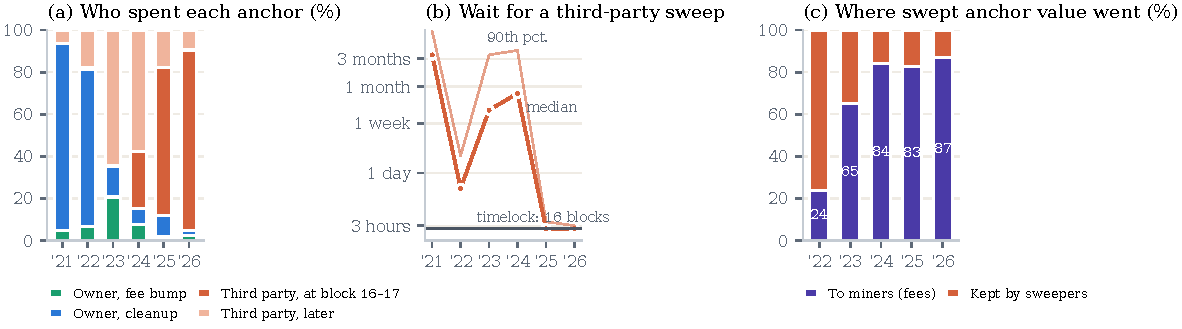
\includegraphics[width=\textwidth]{figures/fig4_anchors.pdf}
\caption{The anchor money trail. (a) Who spent each P2WSH anchor, by year of the force close: its owner in the
commitment's block (fee bump) or later (cleanup), or a third party at blocks 16--17 or later. (b) Wait from the close
to a third-party sweep, public channels: median and 90th percentile (log scale). (c) Where swept anchor value went, by
year of the sweep: fees to miners, or kept by sweepers.}
\label{fig:anchors}
\end{figure*}

\paragraph{No P2WSH anchor is left unspent}
All \AnchorsAll{} P2WSH anchors created by force closes, public or not, at least four weeks before the cutoff had
been spent by the cutoff (Table~\ref{tab:anchors}). Anchors that their owners leave behind
do not stay in the UTXO set: third parties sweep them. That is the premise of an open LND proposal to stop sweeping
them~\cite{lnd8997}. For P2WSH anchors the data confirm it; simple-taproot anchors, below, are the exception.

\paragraph{Owners stopped using their anchors}
Owners spent \OwnerPctTwentyTwo\% of the anchors of 2022's force closes and \OwnerPctTwentySix\% of 2026's
(Fig.~\ref{fig:anchors}a, Table~\ref{tab:anchors}). Most owner spends
were cleanup after the commitment had confirmed, not fee bumps. Bumps peaked in 2023, when owners bumped
\BumpPctNoHtlcTwentyThree\% of anchor force closes without pending HTLCs and \BumpPctHtlcTwentyThree\% of those with
them. Even a same-block child is often not a bump: in 2026, \NotRaisedPctTwentySix\% of them did not raise the
package's fee rate, so they were cleanup that confirmed in the same block.

\paragraph{Sweepers wait for cheap blocks when fees are high}
Anyone may sweep an anchor from the sixteenth block after the close, but when fees were high nobody did so at once. The
median third-party sweep of a public channel's anchor came \ThirdMedDelayTwentyThree{} blocks after a 2023 close,
about \ThirdMedDelayDaysTwentyThree{} days, against exactly \ThirdMedDelayTwentyFive{} from 2025 (Fig.~\ref{fig:anchors}b). For 2023 closes,
\SweepCheaperPctTwentyThree\% of sweeps confirmed in a block cheaper than the one sixteen blocks after the close
(median fee rate \SweepPFiftyAtSweepTwentyThree{} against \SweepPFiftyAtSixteenTwentyThree~sat/vB). The anchors of
2021's closes waited for the cheap blocks of 2022.

\paragraph{Miners take most of the value}
Fees took \MinersShareTwentyTwo\% of the swept anchors' value in 2022, when sweeps paid a median
\SweepMedFrTwentyTwo~sat/vB, and \MinersShareLateMin--\MinersShareLateMax\% from 2024 (Fig.~\ref{fig:anchors}c). From 2022 to the cutoff,
third-party sweeps collected anchors worth \SweepValueBtc~BTC; \SweepMinersBtc~BTC of it went to miners and
\SweepSweepersBtc~BTC to the sweepers. A sweep pays only below \BreakEven~sat/vB, which is why sweepers
wait out high fees.

\paragraph{One operator collects most third-party anchors}
We find \SweepOperators{} sweeping operators from 2022 to the cutoff. Sweeps that give everything to miners, with only
\texttt{OP\_RETURN} outputs, took \SweepBurnPct\% of third-party anchors; of the rest, \SweepOperatorsOverOne{}
operators took more than 1\% each. The largest appeared on \SweepLargestFirst{} and took \SweepLargestPctTwentySix\%
of third-party anchors in 2026 and \SweepLargestPct\% of all since 2022, netting \SweepLargestNetBtc~BTC.

\paragraph{No third party has swept a simple-taproot anchor}
Simple taproot channels' anchors mostly stay unspent. Of \TaprootAnchors{} created from 2023 to the cutoff,
\TaprootAnchorsSpent{} were spent; of the \TaprootAnchorsTwentySix{} created in 2026, \TaprootAnchorsSpentTwentySix.
Every one of those spends is a key-path spend by the anchor's owner, and no input anywhere on the chain spends the
anchor's 16-block script path (\TaprootScriptPathChainwide{} inputs). That path needs the anchor's internal key,
which the commitment does not reveal; the specification has it revealed when the matching \texttt{to\_local} or
\texttt{to\_remote} output is swept~\cite{boltsimpletaproot}. The missing key does not explain the unspent anchors:
for \TaprootKeyExposedUnspent{} of the \TaprootAnchorsUnspent{} unspent anchors the key has been on-chain for a
median of \TaprootKeyExposedDaysMed{} days, and the sweepers that clear P2WSH anchors have not touched them. Why
they do not is a question for the implementations' developers.

\paragraph{The unswept taproot anchors are worth little to a sweeper}
The anchors whose key is on-chain hold \TaprootKeyPublicBtc~BTC in all, less than the largest P2WSH sweeper has
netted (\SweepLargestNetBtc~BTC). Owners' own spends stopped as well, even though adding the anchor to a sweep still
paid: in the first half of 2025, \TaprootCosweepToRemotePctEarly\% of owners' \texttt{to\_remote} sweeps also spent
the matching anchor, against \TaprootCosweepToRemotePctLate\% from July~2026 to the cutoff. The 2026 sweeps paid a
median \TaprootOwnerSweepFrLate~sat/vB, against \TaprootOwnerSweepFrEarly~sat/vB in early 2025, so including the
anchor was worth more to the owner in 2026, not less.
